\documentclass{article}
\usepackage{geometry}
\geometry{
 a4paper,
 total={170mm,257mm},
 left=20mm,
 top=20mm,
}

\usepackage[OT1]{fontenc}
\renewcommand*\familydefault{\sfdefault}

\usepackage{graphicx}
\usepackage[utf8]{inputenc}
\usepackage[english]{babel}
\usepackage[english]{isodate}
\usepackage[parfill]{parskip}
\usepackage[hybrid]{markdown}

\usepackage{xcolor}
\definecolor{ampliproblue}{RGB}{0, 77, 255}
\usepackage{sectsty}
\sectionfont{\color{ampliproblue}}
\subsectionfont{\color{ampliproblue}}
\subsubsectionfont{\color{ampliproblue}}

\markdownSetup{
  pipeTables,
  tableCaptions,
  rendererPrototypes = {
    image = {\begin{center}\setkeys{Gin}{width=.99\linewidth}\includegraphics{#2}\end{center}}, % center images inline expanding to page width
    codeSpan = {\texttt{#1}}, % Render inline code via `\texttt`.'
  }
}
\title{
  \textbf{\raisebox{-0.475em}{
\includegraphics[height=1.65em]{imgs/amplipro_nobg.png}} Expansion Unit - User Manual}
}
\date{}
\setlength\parindent{0pt}
\begin{document}

\maketitle
\setkeys{Gin}{width=.99\linewidth}
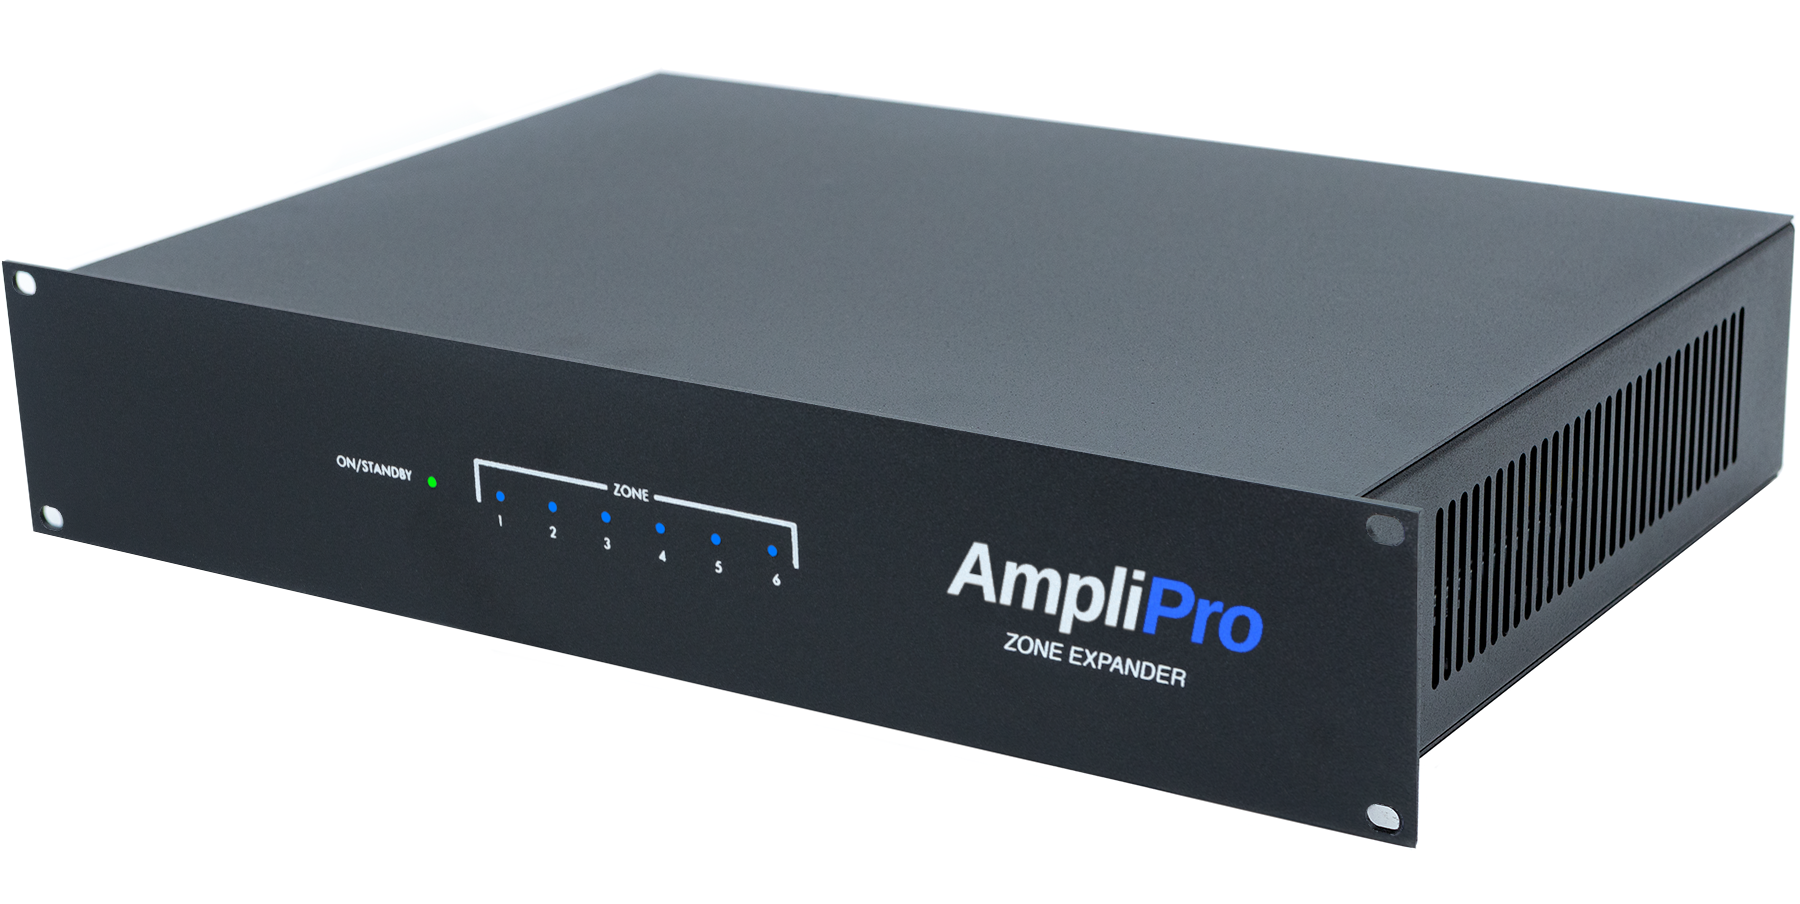
\includegraphics{ expander/sideview_expansion.png}
\begin{center}
  \LARGE{ \textbf{ Device Model: AP1-Z6}}
\end{center}

\includegraphics{ imgs/MicroNova_Logo.jpg}

\thispagestyle{empty}
\newpage
\thispagestyle{empty}
\tableofcontents
\newpage
\pagenumbering{arabic}

\markdownInput{common/LINKS.md}
\newpage
\markdownInput{common/SAFETY.md}
\newpage
\markdownInput{common/FCC.md}
\newpage
\markdownInput{expander/OVERVIEW.md}
\newpage
\markdownInput{expander/ZONE_EXPANDER_SPECS.md}
\newpage
\markdownInput{expander/INSTALLATION.md}
\newpage
\markdownInput{common/TROUBLESHOOTING.md}
\newpage
\markdownInput{common/WARRANTY.md}
\newpage
\markdownInput{common/GLOSSARY.md}

\end{document}
